\documentclass[12pt]{extarticle}
\usepackage[utf8]{inputenc}
\usepackage{cite}
\usepackage{amsmath}
\usepackage{boldline,multirow}
\usepackage{graphicx}
\usepackage{geometry}
\geometry{
a4paper,
left=25mm,
right=25mm,
top=30mm,
bottom=30mm
}


\usepackage{fancyhdr,lastpage}
\graphicspath{{./Images/}}

\pagestyle{fancy}
\fancyhf{}

\setlength{\tabcolsep}{0.7em} % for the horizontal padding
\title{\textbf{Flight Delay Prediction}}
\author{Mahesh Bharadwaj K}
\date{}
\rfoot{Page \thepage \hspace{1pt} of \pageref{LastPage}}
\rhead{Flight Delay Prediction}

\begin{document}
\maketitle
\begin{abstract}
    Flights are said to be delayed when they arrive later than the scheduled arrival time. The delay can be due to several factors including but not limited to adverse weather conditions. The aim of this project is to predict arrival delay of a flight after its departure using a two-stage machine learning model.If the flight is predicted to have an arrival delay, the delay in minutes is predicted.
\end{abstract}
\vfill
\section{Introduction}
The Federal Aviation Authority (FAA) considers flights to be delayed if the arrival delay is greater than 15 minutes. Delays not only agonise the travellers, but also have a domino effect on the background work involving allocation of gates at the airport, ground crew, wastage of food to name a few. This causes losses of billion of dollars to the airline and hence, it is important to predict arrival delays accurately. This project aims to design a two stage model to classify and predict the arrival delay of flights based on the dataset of all flights in USA from 2016 to 2017 and weather data pertaining to 15 selected airports during the same time frame. In this project, the performance of various classification and regression models is studied and compared.
\vfill

\newpage

\section{Dataset}
The flight dataset contains flights from all airports in the USA from 2016 to 2017. The weather dataset contains the weather data obtained from 15 airports in the years 2016 - 2017. The flights for which the weather data is available are selected and the corresponding weather data is appended to the flight data.
 The flight and weather datasets are  merged based on: Departure Airport, Departure Time, and Date.\\
 The Airports for which weather data is available are listed in table \ref{table:1}. The various weather data points considered are given in table \ref{table:2}. The various Flight Performance Metrics considered are given in table \ref{table:3}. There are 18,51,115 data points available in the processed dataset.
 75\% of these data points are designated as training data and the remaining 25\% of the data points are designated as testing data.
\vfill
{\renewcommand{\arraystretch}{1.5}% for the vertical padding
\begin{table}[h]
    \centering
    \begin{tabular}{|c|c|c|c|c|}
    
    \hline
         ATL & CLT & DEN & DFW & EWR\\
    \hline
         IAH & JFK & LAS & LAX & MCO\\
    \hline
        MIA & ORD & PHX & SEA & SFO\\
    \hline
    \end{tabular}
    \caption{\textbf{Airport Codes of the Chosen Airports}}
    \label{table:1}
\end{table}
}
\vfill
{\renewcommand{\arraystretch}{1.5}% for the vertical padding
\begin{table}[h]
    \centering
    \begin{tabular}{|c|c|c|c|}
    \hline
        WindSpeedKmph & WindDirDegree & WeatherCode & PrecipMM\\
    \hline
        Visibility & Pressure & CloudCover & DewPointF\\
    \hline
        WindGustKmph & tempF & WindChillF & Humidity\\
    \hline
        Date & time & SnowFallCM &\\
    \hline
    \end{tabular}
    \caption{\textbf{Weather Data Points Considered}}
    \label{table:2}
\end{table}
}
\vfill
{\renewcommand{\arraystretch}{1.5}% for the vertical padding
\begin{table}[h]
    \centering
    \begin{tabular}{|c|c|c|c|}
        \hline
             FlightDate & Quarter & Year & Month\\
        \hline
            DayofMonth & DepTime & DepDel15 & CRSDepTime\\
        \hline
            DepDelayMinutes & OriginAirport & DestAirport &  \\
        \hline
    \end{tabular}
    \caption{\textbf{Flight Performance Metrics Considered}}
    \label{table:3}
\end{table}
}
\vfill
\newpage

\section{Classification}
The classifier is the first stage of the two-stage model and aims to classify flights as delayed or not. Flights which are delayed have the target variable {\em 'ArrDel15'} = 1 and those which are not have the target variable {\em 'ArrDel15'} = 0. 

\subsection*{Models Used}
\begin{itemize}
    \item Logistic Regression
    \item Decision Tree Classifier
    \item Gradient Boosting Classifier
    \item Random Forest Classifier
\end{itemize}


\subsection*{Performance Metrics for Classifier Models} 
\subsubsection*{Terms used}
\begin{enumerate}
    \item \textbf{TP:} True Positives\\
    Flights Delayed Classified correctly as Delayed
    \item \textbf{FP:} False Positives\\
    Flights On Time Classified as Delayed
    \item \textbf{TN:} True Negatives\\
    Flights Not Delayed correctly classified as Not Delayed
    \item \textbf{FN:} False Negatives\\
    Flights Delayed classified incorrectly as Not Delayed
\end{enumerate}

\subsubsection*{Metrics}
$$\textbf{Accuracy} = \frac{TP + TN}{TP + TN + FP + FN}$$
\\
$$\textbf{Precision} = \frac{TP}{TP + FP}$$
\\
$$\textbf{Recall} = \frac{TP}{TP + FN}$$
\\
$$\textbf{F1 Score} = \frac{2 * Precision * Recall}{Precision + Recall}$$

\newpage

\subsection*{Classifier Performance}
{\renewcommand{\arraystretch}{1.4}% for the vertical padding
\begin{table}[h!]
    \centering
    \begin{tabular}{V{4.0} c V{2.5} c V{2.5} c V{2.5} c V{2.5} c V{2.5} c V{2.5} c V{2.5} c V{4.0}}
    \clineB{1-8}{4.0}
    \multirow{3}{*}{\textbf{Classification Model}} & \multicolumn{7}{c V{4.0}}{\textbf{Performance Metric}}\\
    \clineB{2-8}{2.5}
    {} & \multicolumn{2}{c V{2.5}}{\textbf{Precision}} & \multicolumn{2}{c V{2.5}}{\textbf{Recall}} & \multicolumn{2}{c V{2.5}}{\textbf{F1 Score}} & \multirow{2}{*}{\textbf{Accuracy}}\\
    \clineB{2-7}{2.5}
    {} & 0 & 1 & 0 & 1 & 0 & 1 & {}\\
    \clineB{1-8}{4.0}
    \textbf{Logistic Regression} & 0.92 & 0.89 & 0.98 & 0.68 & 0.95 & 0.77 & 0.92\\
    \clineB{1-8}{2.5}
    \textbf{Decision Tree Classifier}  & 0.92 & 0.68 & 0.91 & 0.71 & 0.92 & 0.69 & 0.87 \\
    \clineB{1-8}{2.5}
    \textbf{Gradient Boosting Classifier}  & 0.92 & 0.90 & 0.98 & 0.69 & 0.95 & 0.78 & 0.92\\
    \clineB{1-8}{2.5}
    \textbf{Random Forest Classifier} & 0.92 & 0.88 & 0.98 & 0.70 & 0.95 & 0.78 & 0.92\\
    \clineB{1-8}{4.0}
    \end{tabular}
    \caption{\textbf{Performance of Classifier Models}}
    \label{table:4}
\end{table}
}

\subsection*{Receiver Operation Characteristics of the Classifiers}
Area under ROC curve is an indicator of the performance of the classifier model trained. Higher the area, better the performance of the model
\begin{itemize}
    \item If the Area $\approx$ 0.5, the model is unable to distinguish between the classes (represented by red line)
    \item If the Area $\approx$ 0.0, the model is predicting the exact opposite of the actual classes
    \item If the Area $\approx$ 1.0, the model is predicting the classes accurately
\end{itemize}
\vfill
\begin{figure}[h]
    \centering
        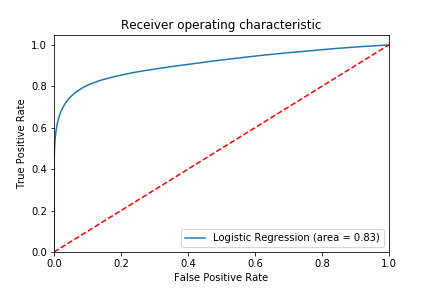
\includegraphics[width=0.45\textwidth]{BeforeSMOTE/LogisticRegressorROC.png}
        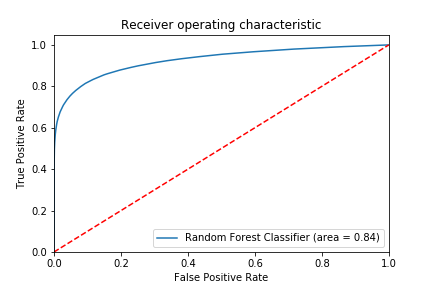
\includegraphics[width=0.45\textwidth]{BeforeSMOTE/RandomForestClassifierROC.png}
    \label{figure:1}
    \caption{\textbf{Logistic Regression \& Random Forest Classifier}}
\end{figure}
\vfill
\newpage

\section{Class Imbalance In Dataset}
The poor performance on class 1 relative to class 0 of the classification algorithms above is due to the inherent bias in the dataset towards non-delayed flights.\\
Out of the 18,51,115 data points in the dataset, only 3,87,948 data points are delayed. The distribution can be seen in figure \ref{figure:2}.

\begin{figure}[h]
    \centering
    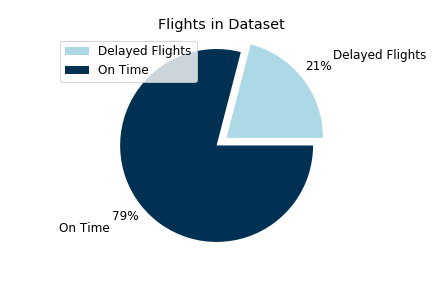
\includegraphics[scale=0.55]{DatasetClassDistributionPieChart.png}
    \caption{\textbf{Pie Chart of Dataset Class Distribution Before SMOTE}}
    \label{figure:2}
\end{figure}

To overcome this bias, there are two options
\begin{itemize}
    \item \textbf{Under Sampling}\\
    The Majority Class is under sampled to ensure there is an even distribution.
    \item \textbf{Over Sampling}\\
    The Minority Class is over sampled to ensure there is an even distribution.
\end{itemize}
Here, Synthetic Minority Oversampling TEchnique referred to as SMOTE has been employed to over-sample the delayed flights. The dataset distribution after SMOTE is given in figure \ref{figure:3}.

\begin{figure}[h]
    \centering
    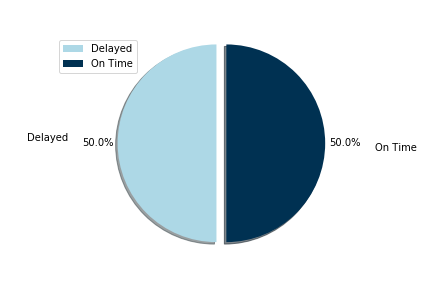
\includegraphics[scale=0.60]{PieAfterSMOTE.png}
    \caption{\textbf{Pie Chart of Dataset Distribution After SMOTE}}
    \label{figure:3}
\end{figure}

\newpage

\subsection*{Classifier Performance After SMOTE}
{\renewcommand{\arraystretch}{1.4}% for the vertical padding
\begin{table}[h!]
    \centering
    \begin{tabular}{V{4.0} c V{2.5} c V{2.5} c V{2.5} c V{2.5} c V{2.5} c V{2.5} c V{2.5} c V{4.0}}
    \clineB{1-8}{4.0}
    \multirow{3}{*}{\textbf{Classification Model}} & \multicolumn{7}{c V{4.0}}{\textbf{Performance Metric}}\\
    \clineB{2-8}{2.5}
    {}  & \multicolumn{2}{c V{2.5}}{\textbf{Precision}} & \multicolumn{2}{c V{2.5}}{\textbf{Recall}} & \multicolumn{2}{c V{2.5}}{\textbf{F1 Score}} & \multirow{2}{*}{\textbf{Accuracy}}\\
    \clineB{2-7}{2.5}
    {} & 0 & 1 & 0 & 1 & 0 & 1 & {}\\
    \clineB{1-8}{4.0}
    \textbf{Logistic Regression} & 0.94 & 0.74 & 0.93 & 0.78 & 0.93 & 0.76 & 0.90\\
    \clineB{1-8}{2.5}
    \textbf{Decision Tree Classifier}& 0.92 & 0.67 & 0.91 & 0.70 & 0.91 & 0.69 & 0.87\\
    \clineB{1-8}{2.5}
    \textbf{Gradient Boosting Classifier}& 0.93 & 0.85 & 0.97 & 0.72 & 0.95 & 0.78 & 0.91\\
    \clineB{1-8}{2.5}
    \textbf{Random Forest Classifier} & 0.93 & 0.83 & 0.96 & 0.73 & 0.95 & 0.78 & 0.91\\
    \clineB{1-8}{4.0}
    \end{tabular}
    \caption{\textbf{Performance of Classifier Models After SMOTE}}
    \label{table:5}
\end{table}
}

\subsection*{Receiver Operation Characteristics After SMOTE}
\begin{figure}[h]
    \centering
        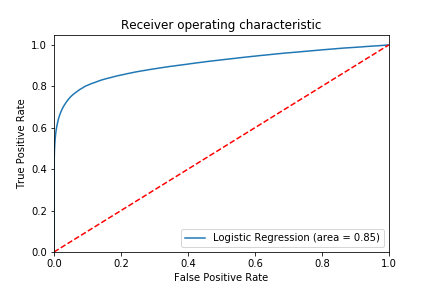
\includegraphics[scale=0.45]{AfterSMOTE/LogisticRegressorROC.png}
    \caption{\textbf{Logistic Regression}}
    \label{figure:4}
        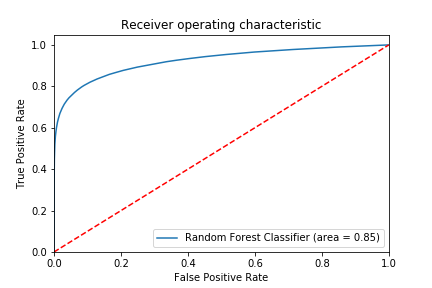
\includegraphics[scale=0.45]{AfterSMOTE/RandomForestClassifierROC.png}
    \caption{\textbf{Random Forest Classifier}}
    \label{figure:5}
\end{figure}

SMOTE oversampling improves the performance of Logistic Regression model by increasing the recall of class 1. Random Forest Classifier and Gradient Boosting Classifier do not show any improvements as they are built to work on imbalanced classes. F1 Score gives equal importance  to precision and recall and hence, the classifier chosen was Random Forest Classifier having the highest F1 Score (0.78).

\newpage

\section{Regression}
Regression is the second stage of the two-stage model. The Arrival Delay in minutes is predicted if the flight is classified as Delayed by the classifier. The flights having {\em 'ArrDelayMinutes'} $>$ 0 are used to train the regression model. The results of the various models used are located in table \ref{table:6}.

\subsection*{Models Used}
\begin{itemize}
    \item Linear Regressor
    \item Gradient Boosting Regressor
    \item Extra Tree Regressor
\end{itemize}

\subsection*{Performance Metrics for Regression Models}
$$\textbf{Mean Squared Error (MSE)} = \frac{1}{n}\sum_{i=1}^{n}(\hat{y_{i}} - y_{i})^{2}$$
$$\textbf{Root Mean Square Error (RMSE)} = \sqrt{\frac{1}{n}\sum_{i=1}^{n}(\hat{y_{i}} - y_{i})^{2}}$$
$$\textbf{Mean Absolute Error (MAE)} = \frac{1}{n}\sum_{i=1}^{n}|\hat{y_{i}} - y_{i}|$$
$$\textbf{\(R^{2}\) Score} = 1 - \frac{\sum_{i=1}^{n}(\hat{y_{i}} -y_{i})^{2}}{\sum_{i=1}^{n}(\hat{y_{i}} - \bar{y})^{2}}$$

{\renewcommand{\arraystretch}{1.4}
\subsection*{Regression Performance}
\begin{table}[h]
    \centering
    \begin{tabular}{V{4.0} c  V{2.5} c V{2.5} c V{2.5} c V{4.0}}
    \clineB{1-4}{4.0}
    \textbf{Regression Model} &  \textbf{RMSE} & \textbf{MAE} & \textbf{\(R^{2}\) Score}\\
    \clineB{1-4}{4.0}
    \textbf{Linear Regression}  & 16.43 & 11.20 & 0.926\\
    \hline
    \textbf{Gradient Boosting Regression} & 15.49 & 10.52 & 0.934\\
    \hline
    \textbf{Extra Tree Regression}  & 15.16 & 10.47 & 0.937\\
    \clineB{1-4}{4.0}
    \end{tabular}
    \caption{\textbf{Regression Performance}}
    \label{table:6}
\end{table}
}

$R^{2}$ Score is a measure of the ability of a model to predict the variances in the dataset accurately. The Regressor chosen was Extra Tree Regressor having $R^{2}$ Score (0.937) and RMSE (15.16). 

\newpage

\section{Regression Analysis}
The arrival delay ranged from 0 to 2142 minutes. Frequency Distribution plot (figure \ref{figure:6}) of the arrival delay reveals that the maximum frequency is observed between 0 - 100 and 100 - 200. The dataset was split into ranges of arrival delay minutes and performance of Linear Regression model is studied in these ranges (table \ref{table:7}).

\begin{figure}[h]
    \centering
    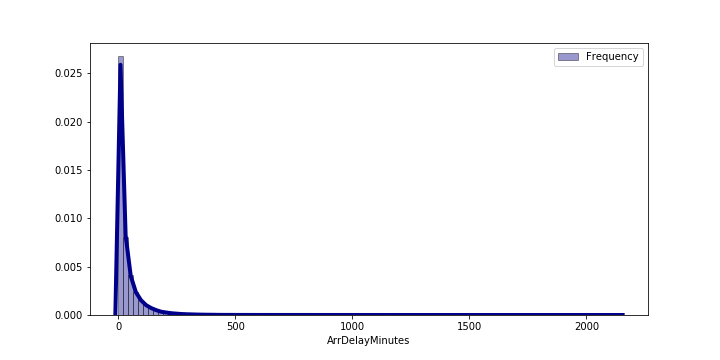
\includegraphics[scale=0.55]{Images/DelayFrequencyHistogram.png}
    \caption{\textbf{Frequency Distribution of Arrival Delay}}
    \label{figure:6}
\end{figure}

{
\renewcommand{\arraystretch}{1.4}
\begin{table}[h]
    \centering
    \begin{tabular}{ V{4.0} c V{2.5} c V{2.5} c V{4.0}}
    \clineB{1-3}{4.0}
    \textbf{Range} & \textbf{RMSE} & \textbf{MAE}\\
    \clineB{1-3}{4.0}
    \textbf{0 - 100}  & 14.51 & 10.44 \\
    \hline
    \textbf{100 - 200}  & 27.50 & 17.74 \\
    \hline
    \textbf{200 - 500}  & 32.34 & 20.15 \\
    \hline
    \textbf{500 - 1000}  & 42.37 & 35.17 \\
    \hline
    \textbf{1000 - 2000}  & 69.53 & 65.55\\
    \clineB{1-3}{4.0}
    \end{tabular}
    \caption{\textbf{Range-wise Regression Analysis}}
    \label{table:7}
\end{table}
}
The results obtained are in line with the frequency distribution histogram. Most data points have {\em 'ArrDelayMinutes'} ranging between 1 - 100 minutes and hence, MAE (10.43) and RMSE (14.51) are least in this range. As the range increases, the number of data points decreases and as result, the values of RMSE and MAE increase.

\newpage

\section{Pipelined Model}
The Classifier chosen is Random Forest Classifier as it has the maximum F1 Score and area under ROC.
The Regression Model chosen in Extra Tree Regressor as it has the highest $R^{2}$ Score.
The Flow Chart given below (figure \ref{figure:7}) is the representation of the two-stage machine learning model built.
\newline
\begin{figure}[h]
    \centering
    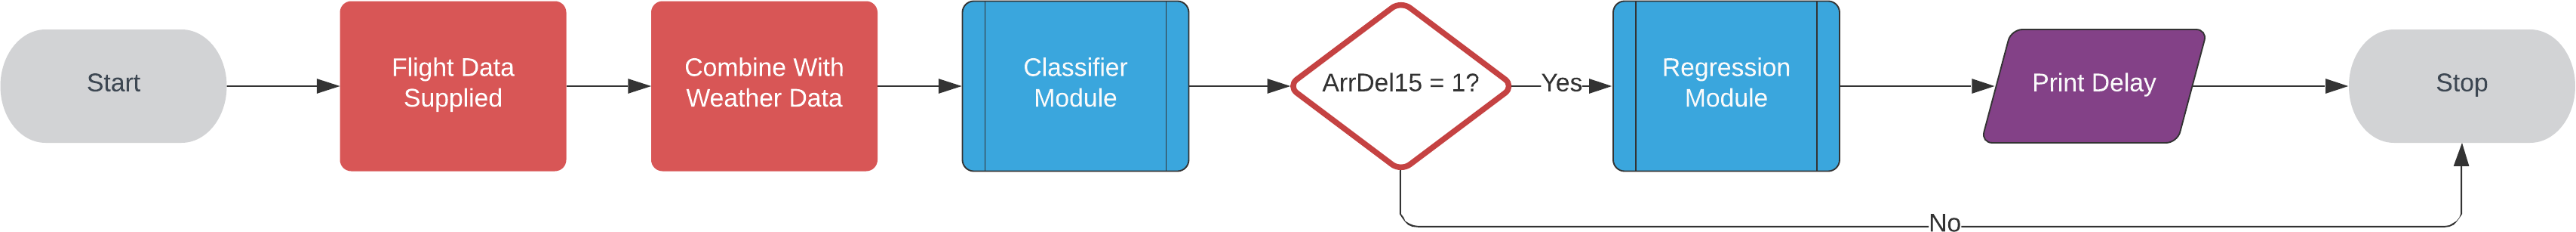
\includegraphics[width=1.0\textwidth]{Flowchart.png}
    \caption{\textbf{Flowchart of Pipelined Model}}
    \label{figure:7}
\end{figure}

\subsection*{Performance of Pipelined Model}

{\renewcommand{\arraystretch}{1.4}
\begin{table}[h]
    \centering
    \begin{tabular}{V{4.0} r V{2.5} c V{4.0}}
        \clineB{1-2}{4.0}
        \textbf{Metric} & \textbf{Value}\\
        \clineB{1-2}{4.0}
        Root Mean Squared Error & 10.74\\
        \hline
        Mean Absolute Error & 7.93\\
        \hline
        $R^{2}$ Score & 0.937\\
        \clineB{1-2}{4.0}
        \end{tabular}
    \caption{\textbf{Pipelined Model Performance}}
    \label{table:8}
\end{table}
}


\section{Conclusion}
The flight and weather data were combined into a single dataset for training the models. It was observed from the classifier that bias in dataset(towards non delayed flights) affected the performance of class 1 relative to class 0 in the classifier models chosen. This bias was overcome by oversampling the delayed flights in the dataset using SMOTE. The Classifier chosen was Random Forest Classifier having the highest F1 Score (0.78) \& Accuracy (0.91).The Regression Model chosen was Extra Tree Regressor having the highest $R^{2}$ Score (0.937) \& least RMSE (15.16) . The pipelined model was designed using the aforementioned Classifier and Regression Models and performed with a good accuracy.

\end{document}

